\documentclass[11pt]{article}
% Shared preamble for the Official Statistics revision notes.
\usepackage[a4paper,margin=0.75in,headheight=14pt]{geometry}
\usepackage{amsmath,amssymb,mathtools}
\usepackage[dvipsnames]{xcolor}
\usepackage{enumitem}
\usepackage{booktabs}
\usepackage{tabularx}
\usepackage{array}
\usepackage{multicol}
\usepackage{tcolorbox}
\usepackage{fancyhdr}
\usepackage{needspace}
\usepackage{tikz}
\usetikzlibrary{arrows.meta,positioning,calc}
\usepackage[colorlinks=true,linkcolor=Blue]{hyperref}
\tcbuselibrary{skins,breakable}

\setlist{itemsep=1pt,topsep=2pt,parsep=0pt}
\setlength{\parskip}{3pt}
\setlength{\parindent}{0pt}
\pagestyle{fancy}\fancyhf{}
\rhead{\small Official Statistics, B.Stat.\ 3rd yr}
\cfoot{\small\thepage}

% Keep a section heading off the foot of a page.
\let\oldsection\section
\renewcommand{\section}{\needspace{9\baselineskip}\oldsection}

\newcommand{\T}[1]{\mathrm{#1}}
\newcommand{\sym}[1]{\mathit{#1}}   % the paper's multi-letter symbols: PE, PHW, ...
\newcommand{\yes}{{\color{ForestGreen}$\checkmark$}}
\newcommand{\no}{{\color{BrickRed}$\times$}}
\newcommand{\df}[1]{\textbf{\color{Blue!75!black}#1}}

% Grey line under each section heading: thrust areas, lectures, past-paper parts answered.
\newcommand{\covers}[3]{{\small\color{black!60}\textsf{Thrust areas #1 \ $\cdot$\ #2 \ $\cdot$\ PYQ: #3}}\par\smallskip}

\tcbset{boxsep=2pt,left=4pt,right=4pt,top=2pt,bottom=2pt,fonttitle=\bfseries\small,breakable,
  before skip=5pt,after skip=5pt}
\newtcolorbox{keybox}[1]{colback=Blue!4,colframe=Blue!60,title={#1}}
\newtcolorbox{trap}[1]{colback=BrickRed!5,colframe=BrickRed!60,title={\textsc{Trap} --- #1}}
\newtcolorbox{tmpl}[1]{colback=Orange!6,colframe=Orange!75!black,title={Numerical template --- #1}}
\newtcolorbox{quick}[1]{colback=ForestGreen!5,colframe=ForestGreen!55,title={Quick check from the slides --- #1}}
\newtcolorbox{pyqbox}[1]{colback=Orange!8,colframe=Orange!80!black,title={#1}}

\lhead{\small Official Statistics --- Midsem Revision Notes}

\begin{document}

\begin{center}
{\LARGE\bfseries Official Statistics}\\[3pt]
{\large Mid-Semester Revision Notes: the System of National Accounts}\\[2pt]
{\small B.Stat.\ 3rd year, Semester V --- Lectures 1--12, keyed to the thrust areas and past papers}
\end{center}
\vspace{1pt}\hrule\vspace{6pt}

These notes cut the 62-page lecture compilation down to what the thrust-area list names, plus
two items the list omits but the 2025--26 paper needs: taxes and subsidies, and residence, which
GNI depends on. The history of economic thought (Lecture 1--2: mercantilists, physiocrats, Smith,
Say) is dropped. It is on neither the list nor any paper.

Each section opens with a grey line giving its thrust areas (T1--T26, numbered as on the list),
its lectures, and the past-paper parts it answers. \textbf{Orange boxes matter most.} The 2025--26
Q2 took two worked examples from the slides and replaced the numbers with symbols. Every slide
example is therefore given here in both forms. Model answers to the paper are in \S\ref{sec:pyq}.

\begin{center}\small
\begin{tabularx}{\textwidth}{@{}c X c l@{}}
\toprule
\textbf{T} & \textbf{Thrust area} & \textbf{\S} & \textbf{Asked in} \\
\midrule
1 & GVA, GVO, GDP, HFCE, IC, GCF, GNI --- definitions and relations & \ref{sec:prod}, \ref{sec:os}, \ref{sec:gni}, \ref{sec:di} & 25--26 Q1(i), (ii), (iv); Q2(i) \\
2, 3 & Two-sector circular flow (real and money flows); $Y=C+I$ & \ref{sec:prod}, \ref{sec:id} & --- \\
4, 5 & Economic flows; exchange, transfer, transactions & \ref{sec:flows} & --- \\
6 & Current and capital transactions & \ref{sec:flows} & 25--26 Q1(viii) \\
7, 8 & General production boundary: inclusion/exclusion; IPP & \ref{sec:boundary} & --- \\
9, 13, 14 & Economically significant prices; market, non-market output, final use & \ref{sec:output} & --- \\
10 & Depreciation, depletion, savings & \ref{sec:dd}, \ref{sec:di} & 25--26 Q1(vi) \\
11 & Purchasers', producers' and basic prices & \ref{sec:prices} & 25--26 Q1(iii) \\
12 & External trade exclusions & \ref{sec:ext} & --- \\
15, 17 & Operating surplus (listed twice) & \ref{sec:os} & 25--26 Q2(i) \\
16 & Earned income & \ref{sec:gni} & 25--26 Q2(ii) \\
18, 19 & Transfers; disposable income & \ref{sec:di} & --- \\
20, 22 & Financial and non-financial assets; inventories & \ref{sec:assets} & 25--26 Q1(v) \\
21 & GDCF, GFCF, HFCE, GFCE & \ref{sec:di}, \ref{sec:assets} & 25--26 Q1(iv) \\
23 & Production, income and expenditure identities & \ref{sec:id} & --- \\
24 & Current account, accumulation account, balance sheet & \ref{sec:seq} & --- \\
25, 26 & Monetary/non-monetary transactions; SNA and MTA & \ref{sec:flows}, \ref{sec:mta} & --- \\
--- & \textit{Not on the list:} taxes and subsidies & \ref{sec:tax} & 25--26 Q1(vii) \\
--- & \textit{Not on the list:} economic territory, residence, exports and imports & \ref{sec:res} & 25--26 Q1(i) \\
\bottomrule
\end{tabularx}
\end{center}

\begin{pyqbox}{How the two past papers line up with this syllabus}
\small
\textbf{2025--26 midsem} (30 marks) fits the thrust areas completely. Q1 is 25 marks: any 5 of 8
pairs, each marked 2.5\,+\,2.5, so define both terms, then state how they are related. Q2 is 5
marks, and both options are slide examples with symbols in place of numbers.

\textbf{2024--25 midsem} asked about SDGs, the health classifications ICD, ICHI, ICF and ESPAR, and
DPSIR and FDES environment statistics. \textbf{None of this is on this year's list or in the notes}.
That paper followed a different syllabus order: its endsem covered FDES, the World Health Survey and
similar topics. Nothing in these notes addresses it.
\end{pyqbox}

\begin{pyqbox}{What to expect this year}
\small \textbf{Q1-type pairs the list names but 2025--26 did not ask:} GDCF and GFCF; market and
non-market output; earned and disposable income; GNI and GNDI; financial and non-financial assets;
exchange and transfer; monetary and non-monetary transactions; current account and accumulation
account; IC and final consumption; rent and rental; economic flows and transactions.\\[2pt]
\textbf{Q2-type slide examples not yet used:} the household's disposable income and saving
(\S\ref{sec:di}); pen and school prices (\S\ref{sec:prices}); the farmer's FCE and saving
(\S\ref{sec:di}); the NPI's borrowing (\S\ref{sec:assets}); the 18,000 economy (\S\ref{sec:prod});
the wallet and household MTA, and the MTA-to-accounts chain (\S\ref{sec:mta}).
\end{pyqbox}

% Sections 1-9: production, flows, boundary, residence, output, prices, external trade, OS, D&D.

%======================================================================
\section{Production, value added and the circular flow}\label{sec:prod}
\covers{T1, T2, T3}{Lectures 1--2}{2025--26 Q1(i), (ii)}

Production is measured without double counting. Marshall's example is a carpet: once the carpet
is counted at full value, the yarn and the labour in it are already counted. A producer is
therefore credited only with the value it \emph{adds}.

\begin{tabularx}{\textwidth}{@{}>{\bfseries}l X@{}}
IC & \df{Intermediate consumption}: goods and services a producer buys and \emph{uses up during} the
production process of the period, such as raw materials, fuel, power, maintenance and hired services. \\
GVO & \df{Gross value of output}: the value of all goods and services the unit produces in the period. \\
GVA & \df{Gross value added} $=$ GVO $-$ IC: the unit's own contribution to production. \\
GDP & \df{Gross domestic product}: the sum of GVA over all resident producers, plus net product taxes.
This is the value of production within the economic territory. \\
HFCE & \df{Household final consumption expenditure}: what resident households spend on goods and
services for final consumption. \\
GCF & \df{Gross capital formation}, or investment: acquisitions less disposals of produced assets,
namely fixed assets (GFCF), change in inventories and valuables. \\
GNI & \df{Gross national income} $=$ GDP $+$ net primary (earned) income from the rest of the world.
This is the income of residents. \\
\end{tabularx}

\begin{keybox}{Relations to reproduce}
\vspace{-8pt}
\begin{align*}
\T{GVA} &= \T{GVO}-\T{IC}, \qquad \T{GVA}_{bp}=\T{GVO}_{bp}-\T{IC}\\
\T{GDP} &= \textstyle\sum \T{GVA}_{bp} + (t-s)_{\text{products}} + (t-s)_{\text{imports}}\\
\T{GVO} &= \T{HFCE}+\T{IC}+\T{GCF}\ \Longrightarrow\ \T{GVA}=\T{HFCE}+\T{GCF},\ \text{i.e. } Y=C+I
  \quad(\text{closed, no govt.})\\
\T{GNI} &= \T{GDP} + \text{net primary income from RoW}, \qquad \text{Net} = \text{Gross} - \T{D\&D}
\end{align*}
\end{keybox}

\subsection*{The two-sector circular flow (T2)}

\begin{center}
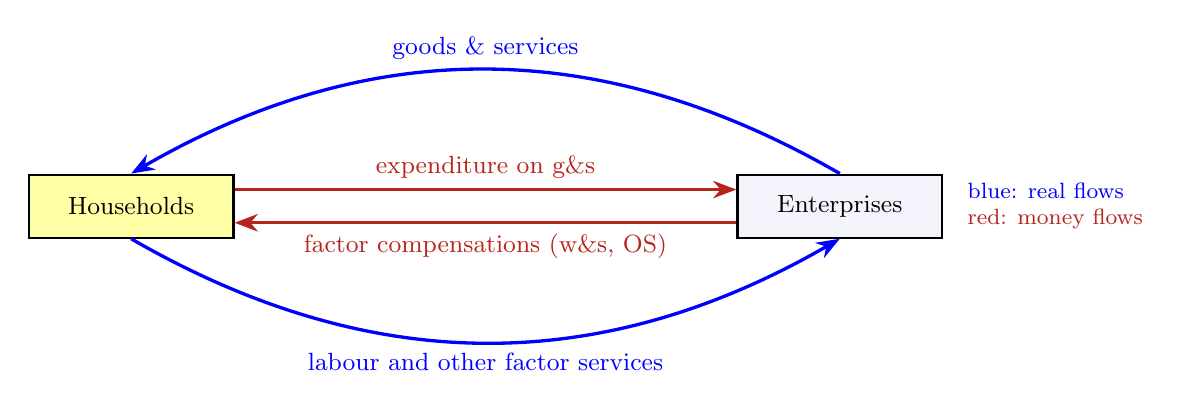
\begin{tikzpicture}[font=\small,>=Stealth,
  box/.style={draw,thick,minimum width=2.6cm,minimum height=0.8cm}]
\node[box,fill=Yellow!35] (H) at (0,0) {Households};
\node[box,fill=Lavender!45] (E) at (9,0) {Enterprises};
\draw[->,very thick,Blue] (E.north) to[out=150,in=30]
  node[midway,above]{goods \& services} (H.north);
\draw[->,very thick,BrickRed] ([yshift=6pt]H.east) --
  node[midway,above]{expenditure on g\&s} ([yshift=6pt]E.west);
\draw[->,very thick,BrickRed] ([yshift=-6pt]E.west) --
  node[midway,below]{factor compensations (w\&s, OS)} ([yshift=-6pt]H.east);
\draw[->,very thick,Blue] (H.south) to[out=-30,in=-150]
  node[midway,below]{labour and other factor services} (E.south);
\node[font=\footnotesize,align=left,anchor=west] at (10.5,0)
  {\textcolor{Blue}{blue: real flows}\\ \textcolor{BrickRed}{red: money flows}};
\end{tikzpicture}
\end{center}

\begin{itemize}
\item Households own \emph{all} factors of production (land, labour, capital, entrepreneurship). They
  sell factor services and are paid factor compensations: wages \& salaries and operating surplus.
  Those payments are the economy's income.
\item Real flows (goods and services, factor services) run opposite to money flows (expenditure,
  compensations).
\item The model rests on Say and Walras: there is no lag between production and income, and no
  income goes unspent. So income equals expenditure (Say's law, ``supply creates its own demand'').
  Keynes (1936) rejected this: spending depends on income, effective demand drives output, and
  aggregate expenditure is $C+I$.
\item Hence \textbf{production $\equiv$ income $\equiv$ expenditure}, which gives the three ways of
  measuring GDP. The \emph{production} approach sums GVA over all producers. The \emph{income}
  approach sums the incomes generated. The \emph{expenditure} approach sums \emph{final}
  expenditure on the goods and services produced.
\end{itemize}

\subsection*{\texorpdfstring{$Y = C + I$}{Y = C + I} (T3)}
The simple circle leaves out enterprise-to-enterprise flows: inputs (IC) and capital goods
(investment). Once they are added, the inputs cancel in aggregation. What remains is
consumption goods plus capital goods, so $Y \equiv C + I_g$. Output left unsold goes into
inventories. The change in inventories (CII) is part of production \emph{and} of investment, so
the identity still holds, and so does $I_g \equiv S$.

\begin{tmpl}{Lecture 2 illustration}
\small Sales 18,000, made up of inputs 3,000, consumption goods 14,000 and capital goods
(tractors) 1,000. Payments: rent 1,200, interest 900, wages \& salaries 8,900.\\
Production $Y = 18{,}000 - 3{,}000 = 15{,}000 = C\,(14{,}000) + I\,(1{,}000)$. Income
$= 8{,}900 + 1{,}200 + 900 + \text{profit }4{,}000 = 15{,}000$, where profit is the residual.\\
\emph{Twist:} households spend only 13,500. Then $S = 15{,}000 - 13{,}500 = 1{,}500$, the 500
unsold goes into CII, and $I_g = 1{,}000 + 500 = 1{,}500 = S$.\\[2pt]
\textbf{Symbolic.} Sales $V$, inputs $N$, consumption goods $C_g$, capital goods $K$:
$Y = V-N = C_g+K$. If households spend $C<C_g$: $\T{CII}=C_g-C$, $S=Y-C$, and $I_g=K+\T{CII}=S$.
\end{tmpl}

\begin{quick}{which are true?}
\small (a) GDP can be measured by production, income and expenditure \yes; (b) production approach
$=$ GVA of all units \yes; (c) income approach $=$ sum of incomes of all households \yes;
(d) expenditure approach $=$ sum of \emph{all} expenditure on goods and services \no, because that
includes IC and only final expenditure counts; (e) total expenditure $=$ FCE $+$ GCF $+$ exports
net of imports \yes.
\end{quick}

%======================================================================
\section{Economic flows and transactions}\label{sec:flows}
\covers{T4, T5, T6, T25}{Lecture 3}{2025--26 Q1(viii)}

An \df{economic flow} is any change in the volume or value of a unit's economic assets. It can be
caused by human acts, by changes in prices, or by natural events. Examples are production, sale
and purchase, taxes, transfers, destruction by calamity, and holding gains.

\begin{multicols}{2}\small
\textbf{Economic flows}
\begin{itemize}
\item \textbf{Transactions}: payments and receipts for production, consumption and accumulation,
  and transfers.
  \begin{itemize}
  \item \df{Exchange}: something is given in return.
  \item \df{Transfer}: nothing is given in return.
  \end{itemize}
\columnbreak
\item \textbf{Other flows}
  \begin{itemize}
  \item \emph{Other changes in volume}: economic value appears or disappears (discoveries,
    destruction by calamity).
  \item \emph{Changes in the level and structure of prices}: holding gains and losses.
  \end{itemize}
\end{itemize}
\end{multicols}

A \df{transaction} is an economic flow in which institutional units interact by mutual agreement.
It can also be an action within one unit that is analytically useful to treat as a transaction,
usually because the unit is acting in two capacities. Transactions are either actual (observed)
or notional (not observable, so imputed). They cover production and exchange of products and
non-produced assets, distribution of income, transfers (current and capital), and financial
assets and liabilities.

\begin{keybox}{Current vs capital transactions (asked: 2025--26 Q1(viii))}
\small
\df{Current transactions} relate to production, final consumption and current transfers:
production-related flows (output, IC, CFC), primary income (CE, OS/MI), production taxes less
subsidies, final consumption, and current transfers such as income taxes and transfers in money
or kind. They do not change the stock of assets directly and are recorded in the \emph{current
accounts}.\\[2pt]
\df{Capital transactions} create or change the volume of a unit's assets: capital formation,
acquisition and disposal of non-produced (natural) assets, capital taxes and capital transfers.
They are recorded in the \emph{accumulation accounts}, and they change the balance sheet.
\end{keybox}

\df{Other perspectives} (T25). A transaction is \emph{between} units or \emph{within} one unit;
within-unit transactions are always non-monetary. It is \emph{monetary} if money changes hands,
and a monetary transaction always has two parties. \emph{Non-monetary} transactions have no
money flow, so they cannot be observed and are imputed, usually at market value. See
\S\ref{sec:mta} for the compiler's tree.

\begin{quick}{economic flows? transactions?}
\small \textbf{Economic flow?} Paddy cultivation \yes; destruction of property by a calamity \yes;
father giving money to his son in the same household \no\ (within one unit); drawing river water
to irrigate land \yes; natural growth of fish stock in a river \no\ (not an economic asset);
price appreciation of real estate \yes.\\
\textbf{Transaction: exchange or transfer?} Production of crops: exchange. Income tax: transfer.
Sale of smuggled goods: exchange (illegal trade still counts). Pickpocketing: transfer. Paying a
lost bet: transfer.
\end{quick}

%======================================================================
\section{The production boundary and IPP}\label{sec:boundary}
\covers{T7, T8}{Lecture 4}{---}

\df{Production} (SNA) is a physical process, under the control and responsibility of an
institutional unit, that uses labour and assets to turn inputs of goods and services into
outputs. The output must be capable of being supplied to another unit, with or without charge.
There are three kinds of product. \emph{Goods} are physical, in demand, and carry ownership that
can be transferred. \emph{Services} change the condition of the consumer or help exchange
products or financial assets (traders, banks). \emph{Data} (2025 SNA) is information produced by
observing phenomena and stored digitally; it is capitalised if used for more than a year, and
then depreciated.

\df{General production boundary}: every activity that one unit could pay another to do for it,
the ``third-person'' test. It excludes only basic human activities such as eating, drinking,
sleeping and taking exercise, which nobody else can do on your behalf.

\begin{keybox}{SNA (2008/2025) production boundary --- inclusion and exclusion}
\small
\begin{tabularx}{\linewidth}{@{}X|X@{}}
\textbf{Included} & \textbf{Excluded} \\ \hline
All \emph{goods}, whether for the market or for own final use (a farmer's crops eaten at home). &
Own-account \emph{household services} by unpaid members: cooking, cleaning, care, repair of own
durables, transporting members. \\
\emph{Services} only if they are sold, supplied to other units, or produced by paid labour (paid
domestic staff). & Volunteer, social and cultural activities. \\
Housing services of owner-occupiers (imputed rent); own-account IPP. & Things that only affect
the quality of life. \\
Non-market output of government and NPISHs; bank services not explicitly charged (FISIM). &
\emph{Theft} (a transfer, not production). \\
Illegal and concealed production (narcotics trade); natural growth of \emph{cultivated} forests. &
Natural growth that nobody manages (wild fish, wild forests). \\
\end{tabularx}
\end{keybox}

\df{Intellectual property products} (T8) are the results of research, innovation and artistic
work. They have been fixed assets since the 2008 SNA. There are four categories: (1) research
and development; (2) mineral exploration and evaluation; (3) computer software, data and
databases; (4) entertainment, literary and artistic originals.

\begin{quick}{inside the SNA boundary? is it production?}
\small \textbf{Inside?} Maintenance and repair of household durables by the household \no; crops
kept for own consumption \yes; owner-occupied housing services \yes; transporting household
members \no; natural growth of cultivated forests \yes; distribution of narcotics \yes.\\
\textbf{Production?} A morning cup of tea \no\ (nothing is created); ploughing \yes; newspaper
delivery \yes\ (trade); repairing a vending machine \yes\ (adds value); natural growth of fish in
a river \no\ (no human effort); collecting wild honey \yes\ (human effort).
\end{quick}

%======================================================================
\section{The domestic economy: territory, units, residence}\label{sec:res}
\covers{--- (background for GNI, exports and imports)}{Lecture 5}{2025--26 Q1(i)}

\begin{itemize}
\item The \df{economy} is all institutional units \emph{resident} in the economic territory during
  the period.
\item The \df{economic territory} is the area the government administers, within which persons,
  goods and capital circulate freely. It includes airspace, territorial waters and continental
  shelf; the country's enclaves abroad (embassies, consulates, military bases, scientific
  stations); and free zones and offshore activity.
\item An \df{institutional unit} can own assets, incur liabilities, carry out economic activity
  and transact with others in its own right. All transactions take place through institutional
  units. A household that also produces is treated as two units, one producing and one consuming.
\item There are \df{five sectors}: non-financial corporations, financial corporations, general
  government, households (including unincorporated enterprises and the informal sector), and
  NPISHs. Government enterprises run like businesses (railways, airlines, power) are
  quasi-corporations and belong in the corporate sector. The central bank is a financial
  corporation.
\item \df{Residence} is the territory where a unit has its \emph{centre of predominant economic
  interest}. It does not depend on nationality or currency. An individual takes the residence of
  their household, and an unincorporated enterprise that of its owner. A corporation or NPI is
  resident where it is registered, and a foreign branch is a resident quasi-corporation of the
  host country. Land and buildings owned by non-residents are assigned a notional resident unit.
  Non-residents that transact with residents form the \df{rest of the world (RoW)}.
\item \df{Exports and imports} are changes of economic ownership between a resident and a
  non-resident.
\end{itemize}

\begin{quick}{export, import or neither (for India)? true or false?}
\small A Kolkata resident buys a Swiss watch in a Kolkata shop: \textbf{N} (the shop is
resident). Online purchase of a UK book: \textbf{M}. An Indian magazine delivered to an Indian
student at Oxford: \textbf{N} (the student is still resident). An Egyptian's hotel bill in
Mumbai: \textbf{X}.\\
Foreign students staying three years are residents \no. A Citibank branch in Kolkata is resident
in India \yes. The Australian crew of a Japanese ship are residents of Japan \no. Non-residents
are not treated as owners of immovable assets \yes. Unincorporated businesses without separate
accounts belong to households \yes. A foreign NPI's branch serving residents is a resident NPISH
\yes. The central bank is in general government \no. A Japanese firm's branch in Thailand is
resident in Thailand \yes.
\end{quick}

%======================================================================
\section{Economically significant prices and the three kinds of output}\label{sec:output}
\covers{T9, T13, T14}{Lectures 5, 7}{---}

\df{Economically significant prices} are prices that significantly affect how much producers are
willing to supply and how much purchasers want to buy. In practice, sales cover the majority of
production costs. General government, the central bank and NPISHs mostly charge nothing or prices
that are not economically significant.

\df{Output} (2025 SNA) is the goods and services an establishment produces. It excludes goods and
services used in an activity where the establishment bears no risk, and those the establishment
consumes itself, unless they are used for own capital formation or own final consumption.

\begin{center}\small
\begin{tabularx}{\textwidth}{@{}l X X X@{}}
\toprule
& \textbf{Market output} & \textbf{Non-market output} & \textbf{Output for own final use} \\
\midrule
What & Sold at economically significant prices & Supplied free, or at prices that are not
economically significant, to other units or the community & Kept by the producer for its own
final consumption or capital formation \\
Who & Corporations, households & General government, NPISHs, central bank (2025 SNA) & Any
producer \\
Valued at & Quantity $\times$ market price & Sum of costs & Market-equivalent price, else sum
of costs \\
Examples & Rented housing, transport corporations, restaurants & Police, free schools run by
trusts, government hospitals & A farmer's own crops, a retailer's own shelves, owner-occupied
housing, paid domestic staff, CII kept for these uses \\
\bottomrule
\end{tabularx}
\end{center}

\df{Sum of costs} (2025 SNA) $=$ IC $+$ remuneration of employees $+$ depreciation (and
depletion) $+$ other taxes less subsidies on production $+$ net return to non-financial assets
$+$ rent on non-produced non-financial assets. Products end up in one of three uses: IC,
consumption of fixed capital (CFC), or \df{final use}, which is final consumption or capital
formation.

\begin{quick}{economically significant? which kind of output?}
\small \textbf{ESP?} Entry ticket to a government museum \no; a pen at the local store \yes; a
restaurant meal \yes; a token OPD registration fee at a free government hospital \no; compulsory
payments by financial corporations to the central bank \no.\\
\textbf{Kind?} Police: non-market. Shelves a retailer builds for his shop: own final use.
Owner-occupied housing: own final use. Rented housing: market. Free schools run by trusts:
non-market. Transport corporations: market.
\end{quick}

%======================================================================
\section{Basic, producers' and purchasers' prices}\label{sec:prices}
\covers{T11}{Lecture 6}{2025--26 Q1(iii)}

A user usually pays more than the producer receives, because of taxes, trade margins and
transport costs. The SNA therefore fixes three valuations:
\begin{itemize}
\item \df{Purchasers' price}: what the purchaser pays to take delivery at the time and place
  required, including trade and transport margins (TTM) and taxes.
\item \df{Producers' price}: what the producer receives from the purchaser, excluding separately
  invoiced VAT and margins.
\item \df{Basic price}: what the producer finally keeps, i.e.\ net of taxes on products and
  including subsidies on products.
\end{itemize}

\begin{keybox}{The price chain}
\centering
Purchasers' price $-$ TTM (and taxes on consumers) $=$ Producers' price\\
Producers' price $-$ (taxes $-$ subsidies) on products $=$ Basic price\\[2pt]
\raggedright\small Output is recorded at \textbf{basic} prices; uses (IC and final use) at
\textbf{purchasers'} prices. The 2008 SNA avoids the term ``market prices'' for value added,
because VAT makes it ambiguous. Write $\T{GDP}=\T{GVA}_{bp}+(t-s)_{\text{products}}$ rather than
``GDP at market prices''.
\end{keybox}

\begin{tmpl}{Lecture 6 pen}
\small A consumer pays 20 to a trader. The trader bought the pen at 12 from the manufacturer,
who paid a product tax of 2. Purchasers' price $=20$; TTM $=20-12=8$; producers' price $=12$;
basic price $=12-2=10$.\\
\textbf{Symbolic.} Consumer pays $p$, trader's cost $q$, product tax $t$, product subsidy $s$:
$\T{TTM}=p-q$; producers' price $=q$; basic price $=q-t+s$.
\end{tmpl}

\begin{tmpl}{Lecture 7 Thai school}
\small A fee of 110 Baht a month from each of 150 students, with a 10\% product tax on the
pre-tax fee, so $110 = 100 + 10$. GVO at producers' prices $=150\times110=16{,}500$; at basic
prices $=150\times100=15{,}000$.\\
\textbf{Symbolic.} $n$ students, fee $f$ including tax at rate $\tau$: producers' $=nf$, basic
$=nf/(1+\tau)$, tax $=nf\tau/(1+\tau)$.
\end{tmpl}

%======================================================================
\section{External transactions and trade exclusions}\label{sec:ext}
\covers{T12}{Lecture 6}{---}

Transactions with the RoW are: exports and imports; primary income (CE and investment income);
current transfers, including taxes on income and wealth; capital transfers; acquisitions less
disposals of valuables and non-produced assets; and financial assets and liabilities.

\begin{itemize}
\item \df{Valuation.} Goods are valued \textbf{f.o.b.} (free on board: excluding insurance and
  freight beyond the exporter's border) at the change of ownership. Customs record imports
  \textbf{c.i.f.} (cost, insurance, freight), but national accounts record imports f.o.b.\ too.
\item \df{Coverage} includes non-residents' spending in the economy (tourists count as exports),
  services such as transport, insurance and hotels, service charges for processing goods owned by
  others, and \df{merchanting}. In merchanting, a merchant in $X$ buys goods from $Y$ and sells
  them to $Z$; ownership changes, but the goods never enter $X$.
\end{itemize}

\begin{keybox}{External trade exclusions (starred in the notes)}
\small \textbf{Rule:} no change of economic ownership between a resident and a non-resident means
no export or import. Excluded:
(1) transactions of non-resident units with the RoW;
(2) flows of samples and goods for exhibition;
(3) goods sent for repair or for rent;
(4) goods of returning residents;
(5) goods sent for processing;
(6) factor services (labour, financial resources), which are primary income, not trade;
(7) goods under operational leasing or rent.
\end{keybox}

\begin{trap}{processing}
\small The \emph{goods} sent abroad for processing are excluded, because the owner never changes.
The processing \emph{fee} is included, as an export of services by the processor's country.
\end{trap}

%======================================================================
\section{Factor incomes, IC, GVA and operating surplus}\label{sec:os}
\covers{T1, T15, T17}{Lectures 5, 7}{2025--26 Q2(i)}

A production process uses labour, inputs (IC), capital goods and natural resources. Part of
the capital goods wears out (depreciation), and part of the non-renewable resources is used up
(depletion). The factors of production are owned, directly or indirectly, by households:

\begin{center}\small
\begin{tabularx}{0.92\textwidth}{@{}l X@{}}
\toprule
\textbf{Factor} & \textbf{Factor payment (compensation)} \\
\midrule
Labour & Compensation of employees, CE (``remuneration of employees'', RE, in 2025 SNA) \\
Land and natural resources & Rent \\
Capital (financial) & Interest \\
Entrepreneurship & Profit \\
A mix of labour and other factors & Mixed income (MI): earnings of unincorporated household enterprises \\
\bottomrule
\end{tabularx}
\end{center}

Rent, interest and profit together make up the \df{operating surplus}.
\begin{itemize}
\item \df{CE / RE}: the total remuneration, in cash or kind, an enterprise owes employees for the
  period's work. It includes wages, salaries, commissions and benefits, \emph{and} the employer's
  social security and PF contributions.
\item \df{Operating surplus (OS)} is the residual once all costs are deducted from output:
  $\T{OS}=\T{GVO}_{bp}-\T{IC}-\T{CE}-\text{other taxes on production (less subsidies)}$. Deduct
  D\&D as well for net OS. OS contains the producer's profit plus the rent and interest paid for
  land and funds owned by others.
\item $\T{GVA}_{bp}$ of corporations and households comes from market output plus output for own
  final use. That of government and NPISHs comes from non-market output plus own final use. For
  the whole economy, $\T{GDP}=\T{GVA}_{bp}+(t-s)_{\text{products}}$.
\end{itemize}

\begin{tmpl}{Lecture 7 bread unit $\to$ asked as 2025--26 Q2(i)}
\small Bread worth 15,000 (without taxes), made from flour 10,000; salaries 1,000; electricity,
fuel and incidentals 2,000.\\
$\T{GVO}_{bp}=15{,}000$; $\T{IC}=10{,}000+2{,}000=12{,}000$; $\T{GVA}_{bp}=3{,}000$;
$\T{OS}=3{,}000-1{,}000=2{,}000$.\\
\textbf{Symbolic} (the exam version: garments $X_1$, fibres $X_2$, salary $X_3$, electricity
etc.\ $X_4$): $\T{GVO}_{bp}=X_1$; $\T{IC}=X_2+X_4$; $\T{GVA}_{bp}=X_1-X_2-X_4$;
$\T{OS}=X_1-X_2-X_3-X_4$.
\end{tmpl}

\begin{trap}{what goes into IC}
\small Salaries are a \emph{factor payment}, never IC. ``Worth (without taxes)'' means basic
prices. \textbf{Factor service, IC or capital good?} Plant and machinery the enterprise owns:
capital good. An office building it hires: IC, since the rental buys a service. Wheat in a flour
mill: IC. Hired land: factor service (rent). A shareholder: factor service. Maintenance of owned
machinery: IC.
\end{trap}

%======================================================================
\section{Depreciation, depletion and gross vs net}\label{sec:dd}
\covers{T10}{Lecture 5}{2025--26 Q1(vi)}

\begin{center}\small
\begin{tabularx}{\textwidth}{@{}l X X@{}}
\toprule
& \textbf{Depreciation} (CFC; called ``depreciation'' in 2025 SNA) & \textbf{Depletion} \\
\midrule
Asset & Produced \emph{fixed} assets & Non-produced \emph{natural} resources (minerals, fuels, wild
stocks) \\
Cause & Wear and tear and normal obsolescence from use in production & Physical removal and
using up by extraction \\
Measures & Cost of fixed capital used up in the period & Natural resources used up in the
period \\
Valued at & \emph{Current} prices of the assets at the time of production, \textbf{not} book
value & Decline in the resource's value \\
In SNA & A cost of production & A cost of production (2025 SNA) \\
\bottomrule
\end{tabularx}
\end{center}

Both reduce the potential to draw benefits from the stock in future. Depreciation can be made good
by new investment; production cannot re-create a depleted natural resource.

\begin{keybox}{Gross $-$ Net $=$ D\&D, for every SNA aggregate}
\centering
NVA $=$ GVA $-$ D\&D; \quad NDP $=$ GDP $-$ D\&D; \quad NNI $=$ GNI $-$ D\&D;\\
net OS $=$ gross OS $-$ D\&D; \quad net profit $=$ gross profit $-$ D\&D; \quad net saving $=$
gross saving $-$ D\&D.
\end{keybox}

\begin{trap}{company depreciation}
\small The depreciation in a company's books is at historic cost, so it is \emph{not} the SNA's
CFC, which is valued at current prices. This is a true/false item in Lecture 12.
\end{trap}

% Sections 10-17: taxes, earned income/GNI, transfers & disposable income, assets & capital
% formation, identities, sequence of accounts, MTA, past-paper answers.

%======================================================================
\section{Taxes and subsidies}\label{sec:tax}
\covers{--- (not on the list, but asked)}{Lecture 4}{2025--26 Q1(vii)}

Government has three economic roles: redistributing income through taxes and subsidies,
non-market production (``general government''), and market production through
quasi-corporations, which sit in the corporate sector.

\begin{itemize}
\item \df{Taxes} are compulsory, unrequited payments, in cash or kind, made to government units
  by households, enterprises and other institutional units.
\item \df{Subsidies} are current, unrequited payments by government \emph{to enterprises only},
  for production activity. They are based on the level of production: quantities or values of
  goods and services produced, sold or imported.
\item \df{Effects.} Taxes raise market prices and leave households and enterprises with fewer
  resources, which lowers private consumption and capital formation. Subsidies do the opposite.
\end{itemize}

\begin{keybox}{Where each kind of tax enters the accounts}
\small
\begin{tabularx}{\linewidth}{@{}l X@{}}
Taxes on products (GST, excise, import duties) & The wedge between basic and producers' prices.
Added to $\T{GVA}_{bp}$ to get GDP. Subsidies on products are the negative wedge. \\
Other taxes on production & Inside $\T{GVA}_{bp}$. Deducted before operating surplus. \\
Current taxes on income and wealth & \emph{Current transfers}. They reduce disposable income, not
GDP or GNI. \\
Capital taxes & \emph{Capital transfers}, in the capital account. \\
\end{tabularx}
\end{keybox}

%======================================================================
\section{Earned (primary) income and GNI}\label{sec:gni}
\covers{T1, T16, T17}{Lecture 8}{2025--26 Q1(i), Q2(ii)}

Household earnings are of two kinds. The first comes from taking part in production. The second
covers everything else: transfers, sale of property and holding gains. Only the first is
\df{earned (primary) income}.

\begin{itemize}
\item \df{Definition.} The income generated in production is the unit's GVA (at producers'
  prices). It is distributed to those who supplied factor services, as factor compensation, and
  to government, as production taxes less subsidies. The recipients' shares are their earned
  (primary) income.
\item \df{Who receives what.} Households and financial institutions receive CE, property income
  (interest and dividends on lent funds, rent on natural resources) and mixed income. Government
  receives taxes less subsidies on production and imports.
\item \df{Property income} is (i) investment income, meaning interest (adjusted for FISIM/IFSLD),
  distributed income of corporations such as dividends, and income on insurance and pension
  entitlements; plus (ii) \df{rent}, the payment for using \emph{non-produced} assets such as land
  or spectrum. A \df{rental} for \emph{produced} assets such as buildings and machinery is the
  purchase of a service, and so counts as IC.
\item Property income paid and received cancels within the domestic economy. That gives the
  \textbf{income approach}: $\T{GDP}=\T{RE}+\T{OS}+\T{MI}+(t-s)_{\text{products}}+(t-s)_{\text{imports}}$,
  with RE counting only what resident enterprises pay.
\item \df{Balance of primary income} $=$ primary income receivable $-$ primary income payable,
  worked out for a unit or a sector.
\item \df{GNI} is the sum of balances of primary income over all residents:
  GNI $=$ GDP $+$ net primary income (CE and property income) from the RoW. \textbf{GDP} measures
  production within the territory. \textbf{GNI} measures the income of residents.
\end{itemize}

\begin{tmpl}{Lecture 8 household $\to$ asked as 2025--26 Q2(ii)}
\small One member works in a factory and another runs a grocery. (a) Salary 5,000; (b) processed
food bought for resale 10,000; (c) remittance from abroad 5,000; (d) contribution to traders'
association 200; (e) income tax 500; (f) sales of processed food 15,000; (g) household provisions
4,350; (h) electricity for the grocery 150; (i) hired worker 1,000; (j) sales tax 150.\\
\textbf{In-flow} $=$ salary $+$ GVA of the grocery $=$ a $+$ (f $-$ b $-$ h) $=5{,}000+4{,}850=9{,}850$.
\textbf{Out-flow} $=$ i $+$ j $=1{,}000+150=1{,}150$. Balance of primary income $=8{,}700$.\\
c, d and e are transfers; g is final consumption. None of them is earned income.
\end{tmpl}

\begin{quick}{earned income? true of GNI?}
\small \textbf{Earned?} Beggars' income \no\ (transfer); smugglers' income \yes\ (illegal trade);
gamblers' income \no\ (transfer); gains from buying and selling shares \no\ (holding gain);
landlord's rent on land \yes; product taxes \yes; sale of land or an existing building \no; income
tax revenue \no\ (transfer).\\
\textbf{GNI?} Includes income tax received from the RoW \no\ (that is GNDI); measures production
\no\ (that is GDP); $=$ GDP $+$ net primary income from the RoW \yes; includes money from a
relative abroad \no; measures the earned income of residents \yes; includes receipts for
consultancy to the RoW \yes; unaffected by domestic production \no.
\end{quick}

%======================================================================
\section{Transfers, disposable income, consumption and saving}\label{sec:di}
\covers{T1, T10, T18, T19, T21}{Lecture 8}{2025--26 Q1(iv)}

\df{Transfers} are one-way: a unit provides goods, services, an asset or money and receives
nothing in return. Capital transfers are covered in \S\ref{sec:assets}.
\df{Current transfers}, other than social transfers in kind, are of three kinds:
\begin{enumerate}
\item current taxes on income, wealth, etc.;
\item \emph{net social contributions and social benefits}. Contributions are paid only by
  households, actual or imputed, and employers' contributions pass through CE first. They are
  received by government and by insurance and pension funds. Benefits are received by households
  when an event occurs: sickness, unemployment, retirement, housing, education, family;
\item \emph{other current transfers}: net non-life premiums and claims, transfers between
  government units (including foreign governments), transfers to and from NPISHs, and transfers
  between households, including remittances.
\end{enumerate}
Insurance premiums are \emph{partly} a payment for the insurer's service; claims are pure transfers.

\begin{quick}{current transfers?}
\small Entirely: corporate tax; election bonds; money sent home by a non-resident; insurance claims
received by a company; a worker's union contribution. Partly: life and non-life premiums. Not
current: a donation to build a school (capital transfer); royalty for a patented design (payment
for a service).
\end{quick}

\begin{keybox}{Disposable income}
\small \textbf{Disposable income} $=$ balance of primary income $+$ current transfers receivable
$-$ current transfers payable, leaving out social transfers in kind. It measures purchasing power.\\
\textbf{GNDI} $=$ GNI $+$ net current transfers from the RoW, including net taxes on income and
wealth $=$ GDP $+$ net primary income from the RoW $+$ net current transfers from the RoW.
\end{keybox}

\begin{tmpl}{Lecture 8 household, continued: the likely next variant}
\small Transfers in $=$ c $=5{,}000$; transfers out $=$ d $+$ e $=700$; net $=4{,}300$.
Disposable income $=8{,}700+4{,}300=13{,}000$. Extension: saving $=$ DI $-$ FCE (g)
$=13{,}000-4{,}350=8{,}650$.\\
\textbf{Symbolic} (2025--26 letters, with $S'$ for the grocery's sales, since the paper uses $S$
twice): $\text{DI}=S+S'-P-\sym{PE}-\sym{PHW}-\sym{PS}+R-\sym{PT}-\sym{PI}$, and saving
$=\text{DI}-\sym{PH}$.
\end{tmpl}

\df{Consumption} is using goods and services up. It takes three forms: \emph{completely} in
production (IC), \emph{partially} in production (CFC, i.e.\ depreciation), or for the direct
satisfaction of needs (\df{final consumption}). Final consumption meets \emph{individual} needs
(a household's own wants) or \emph{collective} needs (services to the whole community). Only
general government and the central bank provide collective services.

\begin{keybox}{HFCE and GFCE (asked: 2025--26 Q1(iv))}
\small
\textbf{Who has FCE:} households, general government, the central bank and NPISHs, but
\emph{never corporations}. $\T{FCE}=\T{PFCE}+\T{GFCE}+\T{CBCE}$, where $\T{PFCE}=\T{HFCE}+$ FCE of
NPISHs.\\[2pt]
\textbf{HFCE}: consumption spending by \emph{resident} households, both in the territory (on
domestic output and imports) and abroad (counted as imports). It includes own-account consumption
such as crops kept and owner-occupied housing. Spending by non-residents in the territory is
exports, not HFCE.\\[2pt]
\textbf{GFCE}: the whole non-market output of general government is treated as consumed by
government itself, even though households enjoy it. Add purchases of market goods passed free to
households, e.g.\ food for flood victims or blankets for the homeless:\\[1pt]
\centerline{$\T{GFCE}=\text{total output of GG}-\text{own-account GCF}-\text{sales of goods and services}
+\text{benefits in kind}.$}
\end{keybox}

\begin{tmpl}{Lecture 8 Malaysian farmer}
\small Mixed income 5,000; rent received 1,000. Grain kept: 100 for seed, 900 to eat. Consumption
goods bought 4,000; fertiliser 500. $\T{FCE}=900+4{,}000=4{,}900$. The seed is inventory, i.e.
next year's IC, and fertiliser is IC.\\
With current transfers of 2,000 and CFC 500: DI $=5{,}000+1{,}000+2{,}000=8{,}000$; gross saving
$=8{,}000-4{,}900=3{,}100$; net saving $=3{,}100-500=2{,}600$.\\
\textbf{Saving:} gross saving $=$ disposable income $-$ FCE (GNDI $-$ FCE for the economy);
net saving $=$ gross saving $-$ D\&D.
\end{tmpl}

%======================================================================
\section{Assets, capital formation and net lending}\label{sec:assets}
\covers{T8, T20, T21, T22}{Lecture 9}{2025--26 Q1(v)}

A \df{financial asset} comes from a contract between two units that gives one of them the right to
a payment, or a series of payments, from the other. Currency, deposits, loans, shares and bonds
are examples. A \df{liability} is the debtor's obligation to pay the creditor. All liabilities are
financial. The payment due is the financial claim, and it ends when the debtor pays.

\begin{keybox}{Non-financial assets (2025 SNA) --- produced vs non-produced (asked: 2025--26 Q1(v))}
\small
\textbf{Produced assets} come into existence as outputs of production:
\begin{itemize}
\item \emph{fixed assets}, used repeatedly in production for more than a year: dwellings, other
  buildings and structures, machinery and equipment, weapons systems, costs of ownership transfer
  on non-produced assets, and IPP;
\item \emph{inventories}: materials and supplies, work in progress, finished goods, military
  inventories, goods for resale;
\item \emph{valuables}, held as stores of value: precious metals and stones, antiques and art,
  jewellery. They are neither consumed nor used in production.
\end{itemize}
\textbf{Non-produced assets} come into existence other than by production: contracts, leases and
licences; purchased goodwill and marketing assets.\\
\textbf{Natural resources}: land, minerals, energy resources (renewable and not), water,
non-cultivated biological resources (non-produced), cultivated biological resources (produced),
and radio spectra (either).\\[2pt]
\textbf{Treatment differs.} Produced fixed assets \emph{depreciate}, and acquiring them is GCF.
Natural resources \emph{deplete}, and acquiring them is recorded separately, not in GCF. The
2008 SNA introduced land improvements, weapons systems and IPP as fixed assets.
\end{keybox}

\begin{keybox}{Capital formation (T21, T22)}
\small
$\T{GDCF}\ (=\T{GCF}) = \T{GFCF} + \T{CII} + \text{acquisitions less disposals of valuables}$.
\begin{itemize}
\item \textbf{GFCF}: acquisitions less disposals of produced fixed assets, whether new or
  existing, and whether bought, bartered, received as capital transfers or made on own account;
  \emph{plus} costs of ownership transfer on non-produced assets; \emph{plus} major improvements
  that extend asset lives. Only GFCF is ``investment'' in the narrow sense.
\item \textbf{CII} $=$ closing stock $-$ opening stock of inventories: unsold finished goods,
  traders' stocks, unused raw materials and work in progress.
\end{itemize}
\end{keybox}

\df{Capital transfers} transfer ownership of a fixed asset, are tied to acquiring or disposing
of one, or forgive a liability. Examples are grants to build a school or temple, debt waivers and
capital taxes. Gross saving plus net capital transfers is usually less than GCF, and the gap is
borrowed:
\begin{center}
Net lending ($+$) / borrowing ($-$) $=$ gross saving $+$ net capital transfers $-$ GCF\\
$-$ net acquisition of non-produced non-financial assets.
\end{center}

\begin{tmpl}{Lecture 9 NPI}
\small A free-education NPI receives donations of 10,000, pays salaries of 7,000, pays no tax, and
has CFC of 200. It gets a capital grant of 50,000 for a classroom costing 100,000.\\
Saving $=10{,}000-7{,}000-200=2{,}800$; funds available $=2{,}800+50{,}000=52{,}800$; it must
borrow $100{,}000-52{,}800=47{,}200$.\\
\textbf{Symbolic.} Donation $D$, salaries $W$, CFC $C$, grant $G$, cost $K$: saving $=D-W-C$;
borrowing $=K-(D-W-C+G)$.
\end{tmpl}
\begin{trap}{CFC is not cash}
\small The slides' 47,200 treats CFC as reducing the funds. Strictly, gross saving is 3,000, so
SNA net borrowing $=100{,}000-3{,}000-50{,}000=47{,}000$. In the exam, follow the slides' working;
if you have time, add a line noting that CFC is non-cash.
\end{trap}

%======================================================================
\section{The main identities}\label{sec:id}
\covers{T3, T23}{Lectures 2, 9}{---}

\begin{keybox}{Three approaches to GDP}
\vspace{-8pt}
\begin{align*}
\text{Production:}\quad \T{GDP} &= \T{GVO}_{bp}-\T{IC}+(t-s)_{\text{products}}+(t-s)_{\text{imports}}\\
\text{Income:}\quad \T{GDP} &= \T{RE}+\T{OS}+\T{MI}+(t-s)_{\text{products}}+(t-s)_{\text{imports}}\\
\text{Expenditure:}\quad \T{GDP} &= \T{PFCE}+\T{GFCE}+\T{CBCE}+\T{GFCF}+\T{CII}+\text{valuables}+X-M
\end{align*}
\end{keybox}

\textbf{The eight numbered identities (Lecture 9)}, which underlie the sequence of accounts:
\begin{enumerate}[label={[\arabic*]},leftmargin=2.2em]
\item \emph{Commodity balance}: $\T{GVO}+M \equiv \T{IC}+\T{PFCE}+\T{GFCE}+\T{CBCE}+\T{GFCF}+\T{CII}+\text{valuables}+X$.
  Everything produced or imported is used.
\item \emph{Production}: $\T{GDP}\equiv\T{GVO}_{bp}-\T{IC}+(t-s)_{\text{products}}+(t-s)_{\text{imports}}$.
\item \emph{Income}: $\T{GDP}\equiv(\T{RE}+\T{OS}+\T{MI})$ generated in domestic enterprises
  $+\,(t-s)_{\text{products}}+(t-s)_{\text{imports}}$.
\item \emph{National income}: GNI $\equiv$ [3] $+$ net RE from the RoW $+$ net property income
  from the RoW.
\item \emph{Disposable income}: GNDI $\equiv$ GNI $+$ net current transfers $+$ net taxes on
  income and wealth from the RoW.
\item \emph{Expenditure}: $\T{GDP}\equiv\T{PFCE}+\T{GFCE}+\T{CBCE}+\T{GFCF}+\T{CII}+\text{valuables}+X-M$.
\item \emph{Saving}: $\text{Gross saving}\equiv\T{GNDI}-\T{PFCE}-\T{GFCE}-\T{CBCE}$.
\item \emph{Net lending}: $\equiv$ gross saving $+$ net capital transfers $-(\T{GFCF}+\T{CII}+\text{valuables})$
  $-$ net acquisition of non-produced non-financial assets.
\end{enumerate}

\df{Commodity-flow identity} (Lecture 2), with both sides at purchasers' prices:
\[
\T{GVA}_{bp}+(t-s)_{\text{products}}+M+\text{import duties}=\T{HFCE}+\T{GCF}+X,
\qquad\text{i.e.}\qquad Y+M=C+I+X.
\]

\begin{keybox}{The ladder of aggregates}
\small
\begin{tabularx}{\linewidth}{@{}r X r@{}}
& GDP & \\
$+$ & net primary (earned) income from RoW & $=$ \textbf{GNI} \\
$+$ & net current transfers (incl.\ taxes on income and wealth) from RoW & $=$ \textbf{GNDI} \\
$-$ & final consumption expenditure & $=$ \textbf{Gross saving} \\
$+$ & net capital transfers from RoW $-$ GCF $-$ net acquisition of non-produced assets &
$=$ \textbf{Net lending/borrowing} \\
\end{tabularx}\\[2pt]
Subtract D\&D from any of GDP, GNI, GNDI or saving to get the net version.
\end{keybox}

\begin{trap}{D\&D in the last rung}
\small The Lecture 9 summary slide also subtracts D\&D in the final step. That is only right if
you start from \emph{net} saving and use \emph{net} capital formation (GCF $-$ D\&D). Starting
from gross saving, do \emph{not} subtract D\&D. The Lecture 12 capital account confirms this:
gross saving $33+10=43$, and $43+1-2-23=19$.
\end{trap}

%======================================================================
\section{The sequence of accounts and balance sheets}\label{sec:seq}
\covers{T24}{Lecture 10}{---}

The SNA records all flows and stocks. Accounts are compiled for each of the five sectors, the RoW
and the total economy. They are consistent because there is one production boundary and one asset
boundary. There are three classes:
\begin{enumerate}
\item \df{Current accounts} record production, income and its use. They do not change the balance
  sheet directly. They are the \emph{production account} and the \emph{income accounts}:
  generation of income, allocation of primary income, secondary distribution (income transfers
  other than social transfers in kind), and use of disposable income.
\item \df{Accumulation accounts} record changes in assets and liabilities: the \emph{capital
  account} (capital formation, capital transfers, non-produced assets) and the \emph{financial
  account} (all transactions in financial assets and liabilities). Other changes in volume and
  revaluation also belong here but are not in this course.
\item \df{Balance sheets} record stocks at the opening and closing of the period. Assets
  (produced, non-produced, financial) sit on the left; liabilities (all financial) and net worth
  on the right. \textbf{Net worth} $=$ total assets $-$ total liabilities, the measure of wealth.
  Closing balance sheet $=$ opening balance sheet $+$ transactions $+$ other flows.
\end{enumerate}

\begin{center}\small
\begin{tabular}{@{}lll@{}}
\toprule
\textbf{Account type} & \textbf{Left side} & \textbf{Right side} \\
\midrule
Current accounts & Uses (``expenditures'') & Resources (``revenues'') \\
Accumulation accounts & Changes in assets & Changes in liabilities and net worth \\
Balance sheet & Assets & Liabilities and net worth \\
\bottomrule
\end{tabular}
\end{center}

Every account is a T-account under double entry, so its two sides total the same. The
\df{balancing item} is resources minus uses, shown on the uses side. It is carried forward as the
first resource of the next account. The balancing items are the headline aggregates: GDP/NDP,
OS/MI, GNI/NNI, disposable income, saving, and net lending/borrowing. The full worked chain is in
\S\ref{sec:mta}.

%======================================================================
\section{Monetary transactions and the MTA}\label{sec:mta}
\covers{T25, T26}{Lectures 11--12}{---}

\textbf{The compiler's view.} Two-party transactions can usually be observed. Intra-unit
transactions, some non-produced items, and \emph{composite} financial transactions (one payment
that bundles several analytically different transactions) cannot, so they are imputed or derived.

\begin{multicols}{2}\small
\df{Monetary transactions}: money changes hands, always between two units, and they are recorded
as observed. The exception is composite ones such as nominal interest and total insurance
premiums, which are split into components (FISIM).
\begin{itemize}
\item Goods and services, produced or non-produced (g\&s $\leftrightarrow$ money);
\item distributive: earned income (factor services $\leftrightarrow$ money) and transfers
  (money $\to$ nothing);
\item financial (money $\leftrightarrow$ money), simple or composite.
\end{itemize}
\columnbreak
\df{Non-monetary transactions}: no money flows, so they cannot be observed. They are imputed at
market-equivalent prices, or at the sum of costs if there is no market.
\begin{itemize}
\item \emph{Two-party}: barter and payments in kind; transfers in kind;
\item \emph{intra-unit}: production for own final use (own-account capital formation, own
  consumption), and D\&D.
\end{itemize}
\end{multicols}

\begin{keybox}{Money balance identity}
\centering money in-flow $\equiv$ money out-flow $+$ change in cash in hand\\[1pt]
\raggedright\small Wallet: starts with 100; lunch 20, transport 30, client pays 150, loan from a
friend 350, stationery 500. In-flow 500, out-flow 550, change $-50$, leaving 50.
\end{keybox}

\begin{multicols}{2}\small
\textbf{In-flows} come from selling products, receiving factor and property income, receiving
transfers, \emph{incurring liabilities} (taking a loan, issuing shares or bonds), and
\emph{disposing of financial assets}.\\
\columnbreak
\textbf{Out-flows} go to buying products, paying income, paying transfers, \emph{extinguishing
liabilities} (repaying a loan, buying back shares), and \emph{acquiring financial assets}
(deposits, shares, bonds). Cash is a financial asset.
\end{multicols}

\begin{tmpl}{Lecture 11 household MTA}
\small Sold produce 240, bought goods and services 200, received wages 20, paid wages 80, received
remittances 10, paid transfers 2, borrowed 100. In-flow 370, out-flow 282, so financial assets
rose by 88.\\[2pt]
\centering
\begin{tabular}{@{}rl|lr@{}}
\toprule
\multicolumn{2}{c|}{\textbf{Expenditures}} & \multicolumn{2}{c}{\textbf{Revenues}} \\
\midrule
200 & Bought products & Sold products & 240 \\
80 & Paid income & Received income & 20 \\
2 & Paid transfers & Received transfers & 10 \\
88 & Change in financial assets (incl.\ cash) & Change in liabilities & 100 \\
\midrule
370 & Total & Total & 370 \\
\bottomrule
\end{tabular}
\end{tmpl}

\begin{itemize}
\item \df{Double entry.} Every monetary transaction affects two cells of a unit's MTA. A tractor
  (40) bought with a bank loan is ``bought products 40'' and ``change in liabilities 40''. Wages
  (10) paid into a bank account are ``received income 10'' and ``change in financial assets 10''.
  Each transaction has two parties, so the system as a whole records it four times
  (\df{quadruple entry}).
\item \df{Aggregation} adds corresponding cells. Among residents only, products sold $\equiv$
  bought, income receivable $\equiv$ payable, transfers receivable $\equiv$ payable, and change
  in liabilities $\equiv$ change in financial assets.
\item \df{With the RoW}, the two sides no longer match item by item:
  products sold $+$ imports $\equiv$ products bought $+$ exports, and so on. The one identity
  that holds for \emph{every} sector and for the RoW is
  \begin{center}
  sub-total non-financial (revenue) $+$ change in liabilities\\
  $\equiv$ sub-total non-financial (expenditure) $+$ change in financial assets,
  \end{center}
  so \textbf{non-financial balance $=$ net lending $=$ change in financial assets $-$ change in
  liabilities}.
\end{itemize}

\begin{center}\small
\begin{tabular}{@{}rl|lr|r@{}}
\toprule
\multicolumn{2}{c|}{\textbf{Expenditure}} & \multicolumn{2}{c|}{\textbf{Revenue}} & \textbf{Rev $-$ Exp} \\
\midrule
1235 & Bought products & Sold products & 1259 & 24 \ ($=X-M$) \\
404 & Paid income & Received income & 400 & $-4$ \\
5 & Paid transfers & Received transfers & 4 & $-1$ \\
1644 & \textit{Sub-total non-financial} & \textit{Sub-total non-financial} & 1663 & \textbf{19} \\
203 & Change in financial assets & Change in liabilities & 184 & $-19$ \\
\bottomrule
\end{tabular}
\end{center}
This is the aggregated MTA of all residents (Lecture 11), and it shows the economy is a
\textbf{net lender of 19}. The same identity holds sector by sector in the Lecture 12 table.
Households: $405+4=401+8$, so they lend 4. RoW: $323-342=-19$, so the RoW borrows the 19.

\df{From the MTA to the SNA accounts} (Lecture 12). The MTA records only monetary transactions and
does not say what purchases were for. Extending it takes three steps: split it by sector; add the
non-monetary transactions (own-use output 23, non-market output 43, so $\T{GVO}_{mp}=1259+23+43=1325$);
and break the broad items down. Use of products, 1301, splits into IC 870, FC 408 and CF 23.
Income splits into RE, property income and $(t-s)$. Transfers split into current and capital. With
D\&D $=10$:

\begin{center}\small
\begin{tabularx}{\textwidth}{@{}l X l@{}}
\toprule
\textbf{Account} & \textbf{Resources $-$ uses} & \textbf{Balancing item} \\
\midrule
\multicolumn{3}{@{}l}{\textit{Current accounts}} \\
Production & GVO$_{mp}$ 1325 $-$ IC 870 & GDP 455; NDP 445 \\
Generation of income & NDP 445 $-$ RE paid 153 $-$ production $(t-s)$ and import duties 130
  & OS $+$ MI (net) 162 \\
Allocation of primary income & 162 $+$ RE received 152 $+$ PI received 118 $+$ $(t-s)$ 130
  $-$ PI paid 121 & NNI 441 \\
Secondary distribution & 441 $+$ current transfers received 3 $-$ current transfers paid 3
  & NNDI 441 \\
Use of disposable income & 441 $-$ final consumption 408 & net saving 33 \\
\midrule
\multicolumn{3}{@{}l}{\textit{Accumulation accounts}} \\
Capital & 33 $+$ capital transfers received 1 $-$ paid 2 $-$ (GCF 23 $-$ D\&D 10)
  & net lending 19 \\
Financial & change in financial assets 203 $-$ change in liabilities 184 & net lending 19 \\
\bottomrule
\end{tabularx}
\end{center}
Check by expenditure: $408+23+24=455=$ GDP. Net lending is the \emph{same} 19 as the MTA balance,
because each non-monetary item enters both sides.

\begin{keybox}{Rules of accounting (Lecture 12)}
\small \textbf{Valuation.} Monetary exchanges are valued at the price the buyer actually paid.
Non-monetary ones use market-price equivalents, or the sum of costs where there is no market.
Exports and imports are f.o.b. Flows and stocks are both at current market value.\\
\textbf{Timing.} Products and financial assets are recorded when economic ownership changes.
Primary income and transfers are recorded when they fall due (accrual). Output and IC are
recorded when production takes place. Both parties must record the same value in the same period.
\end{keybox}

\begin{quick}{Lectures 11--12 true/false}
\small Cash in hand is not a financial asset \no. Every monetary transaction makes at least two
entries in a unit's MTA \yes. The MTA records stocks of assets \no. Unequal MTA totals mean a
missing entry \yes. Borrowing is a money in-flow \yes. In an open economy, products bought equal
products sold \no. The non-financial balance is net lending \yes. Money lent between residents
cancels out \yes. The MTA records detailed production, consumption and accumulation \no. All
transaction identities fail for sector accounts \no. The RoW account is presented from the
non-residents' point of view \yes. Net lending is affected by non-monetary transactions \no. Crop
output for own use is recorded in the use-of-income account \yes. Import duties are in the
production account \yes. All non-monetary transactions are valued at cost \no. Primary income and
transfers are on an accrual basis \yes.
\end{quick}

%======================================================================
\section{Past papers: model answers}\label{sec:pyq}

\subsection*{2025--26 Q1 --- define and relate, any 5 of 8 \hfill [(2.5 + 2.5) $\times$ 5 = 25]}
Give all eight a look, then pick the five you can write fastest. The shape of each answer:
define the first term, define the second, and give the relation, preferably as an equation.

\textbf{(i) GNI and GDP.} \emph{GDP} is the value of production by resident producers in the
economic territory during the period: $\sum\T{GVA}_{bp}+(t-s)_{\text{products}}+(t-s)_{\text{imports}}$.
It can also be computed as $\T{RE}+\T{OS}+\T{MI}+(t-s)$, or as $\T{PFCE}+\T{GFCE}+\T{CBCE}+\T{GCF}+X-M$.
\emph{GNI} is the sum of the balances of primary income of all residents, i.e.\ their earned
income. The relation is $\T{GNI}=\T{GDP}+$ (CE $+$ property income) received from the RoW $-$
(CE $+$ property income) paid to the RoW. GDP is a \emph{territorial production} concept and GNI
a \emph{residents' income} concept. Remittances and income taxes from abroad are transfers, so
they enter GNDI, not GNI. $\T{NNI}=\T{GNI}-\T{D\&D}$. [\S\ref{sec:prod}, \S\ref{sec:gni}]

\textbf{(ii) GVA and GVO.} \emph{GVO} is the value of the goods and services an establishment
produces in the period. Market output is valued at basic prices (quantity $\times$ price);
non-market and own-use output at the sum of costs. It includes changes in inventories of finished
goods and work in progress, and own-account capital formation. \emph{GVA} $=$ GVO $-$ IC, the
value the unit itself adds. It is shared out as CE $+$ OS/MI $+$ other net taxes on production.
Summing $\T{GVA}_{bp}$ over residents and adding net product taxes gives GDP; NVA $=$ GVA $-$
D\&D. [\S\ref{sec:prod}, \S\ref{sec:os}]

\textbf{(iii) Basic, producers' and purchasers' prices.} Define all three (\S\ref{sec:prices}) and
give the chain. Purchasers' price $-$ TTM $=$ producers' price. Producers' price $-$ (taxes $-$
subsidies) on products $=$ basic price. Output is valued at basic prices and uses at purchasers'
prices. Illustrate with the pen: 20, then 12, then 10.

\textbf{(iv) HFCE and GFCE.} Use the definitions in the box in \S\ref{sec:di}. The relation:
both are parts of FCE, with $\T{FCE}=\T{PFCE}+\T{GFCE}+\T{CBCE}$, and they enter
$\T{GDP}=\T{PFCE}+\T{GFCE}+\T{CBCE}+\T{GCF}+X-M$. Households \emph{consume} most government
output, but the \emph{expenditure} is recorded as government's. Corporations never have FCE.

\textbf{(v) Produced and non-produced assets.} Produced assets arise from production: fixed
assets, inventories, valuables. Non-produced assets arise otherwise: natural resources such as
land, minerals and water; contracts, leases and licences; goodwill. The treatment differs.
Produced fixed assets depreciate and their acquisition is GCF. Non-produced natural resources
deplete and their acquisition is a separate capital-account item. [\S\ref{sec:assets}]

\textbf{(vi) Depletion and depreciation.} Use the table in \S\ref{sec:dd}: which asset each
applies to, what causes it, current-price valuation, and that both are costs of production.
Then state $\text{Gross}-\text{Net}=\T{D\&D}$.

\textbf{(vii) Taxes and subsidies.} Give both definitions from \S\ref{sec:tax}: compulsory and
unrequited, versus current unrequited payments to enterprises only, based on the level of
production. Then the relation: product $(t-s)$ is the gap between producers' and basic prices, and
$\T{GDP}=\T{GVA}_{bp}+(t-s)_{\text{products}}$. Income taxes are current transfers, and taxes
raise prices while subsidies lower them.

\textbf{(viii) Transactions of current and capital nature.} Use the box in \S\ref{sec:flows}.
Current transactions involve production, primary income, final consumption and current transfers,
and go in the current accounts. Capital transactions involve capital formation, non-produced
assets, capital transfers and capital taxes, go in the accumulation accounts, and change the
balance sheet.

\subsection*{2025--26 Q2 --- answer one \hfill [5]}

\textbf{(i) Textile unit.} Garments $X_1$ (without taxes), fibres $X_2$, salaries $X_3$,
electricity and other incidentals $X_4$. [1 $+$ 2 $+$ 2]
\begin{align*}
\T{GVO}_{bp} &= X_1 \quad \text{(``without taxes'' means basic prices)}\\
\T{IC} &= X_2+X_4\\
\T{OS} &= \T{GVA}_{bp}-\T{CE}=(X_1-X_2-X_4)-X_3=X_1-X_2-X_3-X_4
\end{align*}
State the assumptions: no other taxes on production, and OS is gross, i.e.\ before depreciation.
Salaries are a factor payment, not IC.

\textbf{(ii) Household.} The paper uses $S$ both for salary (a) and for sales (f). Call the sales
$S'$ and \emph{say so in your answer}. [3 $+$ 2]
\begin{align*}
\text{In-flow} &= S+(S'-P-\sym{PE}) && (\text{salary} + \text{GVA of the grocery})\\
\text{Out-flow} &= \sym{PHW}+\sym{PS} && (\text{CE paid} + \text{product tax})
\end{align*}
Excluded: $R$, $\sym{PT}$ and $\sym{PI}$ are current transfers, and $\sym{PH}$ is final
consumption. The balance of primary income is $S+S'-P-\sym{PE}-\sym{PHW}-\sym{PS}$. The slide
numbers give 9,850, 1,150 and 8,700.


\end{document}
